%\documentstyle[epsf,twocolumn]{jarticle}       %LaTeX2e仕様
%\documentclass[twocolumn]{jarticle}     %pLaTeX2e仕様(platex.exeの場合)
\documentclass[onecolumn]{ujarticle}   %pLaTeX2e仕様(uplatex.exeの場合)
%%%%%%%%%%%%%%%%%%%%%%%%%%%%%%%%%%%%%%%%%%%%%%%%%%%%%%%%%%%%%%
%%
%%  基本バージョン
%%
%%%%%%%%%%%%%%%%%%%%%%%%%%%%%%%%%%%%%%%%%%%%%%%%%%%%%%%%%%%%%%%%
\setlength{\topmargin}{-45pt}
%\setlength{\oddsidemargin}{0cm}
\setlength{\oddsidemargin}{-7.5mm}
%\setlength{\evensidemargin}{0cm}
\setlength{\textheight}{24.1cm}
%setlength{\textheight}{25cm}
\setlength{\textwidth}{17.4cm}
%\setlength{\textwidth}{172mm}
\setlength{\columnsep}{11mm}

%\kanjiskip=.07zw plus.5pt minus.5pt

% 【節が変わるごとに (1.1)(1.2) … (2.1)(2.2) と数式番号をつけるとき】
%\makeatletter
%\renewcommand{\theequation}{%
%\thesection.\arabic{equation}} %\@addtoreset{equation}{section}
%\makeatother

%\renewcommand{\arraystretch}{0.95} 行間の設定
%%%%%%%%%%%%%%%%%%%%%%%%%%%%%%%%%%%%%%%%%%%%%%%%%%%%%%%%
%\usepackage{graphicx}   %pLaTeX2e仕様(\documentstyle ->\documentclass)
\usepackage[dvipdfmx]{graphicx}
\usepackage{subcaption}
\usepackage{multirow}
\usepackage{amsmath}
\usepackage{url}
\usepackage[bb=boondox]{mathalfa}
\usepackage{listings}
\newcommand{\argmax}{\mathop{\rm arg~max}\limits}
\newcommand{\argmin}{\mathop{\rm arg~min}\limits}

\lstset{%
  language={Python},
  basicstyle={\small},%
  identifierstyle={\small},%
  commentstyle={\small\itshape},%
  keywordstyle={\small\bfseries},%
  ndkeywordstyle={\small},%
  stringstyle={\small\ttfamily},
  frame={tb},
  breaklines=true,
  columns=[l]{fullflexible},%
  numbers=left,%
  xrightmargin=0zw,%
  xleftmargin=3zw,%
  numberstyle={\scriptsize},%
  stepnumber=1,
  numbersep=1zw,%
  lineskip=-0.5ex%
}

%%%%%%%%%%%%%%%%%%%%%%%%%%%%%%%%%%%%%%%%%%%%%%%%%%%%%%%%
\begin{document}

	%bibtex用の設定
	%\bibliographystyle{ujarticle}
	\noindent

	\hspace{1em}
	2020 年 10 月 16 日
	ゼミ資料
	\hfill
	M2 寺内 光

	\vspace{2mm}

	\hrule

	\begin{center}
		{\Large \bf 進捗報告}
	\end{center}

	\hrule
	\vspace{3mm}

	% ‚ここから 文章 Start!
	\section{今週やったこと}
	\begin{itemize}{
    \item{個体数変化の実験}
    \item{エントロピーと最終拡張の選択個数の確認}
	}\end{itemize}

  \section{個体数変化の実験}
  Translate 修正後,最終個体数(最終拡張数) $B$ を変化させる実験をした.図 \ref{fig:change_B} に結果を示す.
  最終個体数が増えるごとに識別率の上昇が確認できた. 実験で用いた $B$=16 における識別率より $B$=20 における識別率のほうが高くなったが,個体数が増えすぎるとぶれも大きくなる傾向が見られた.

  \begin{figure}[ht]
    \begin{center}
      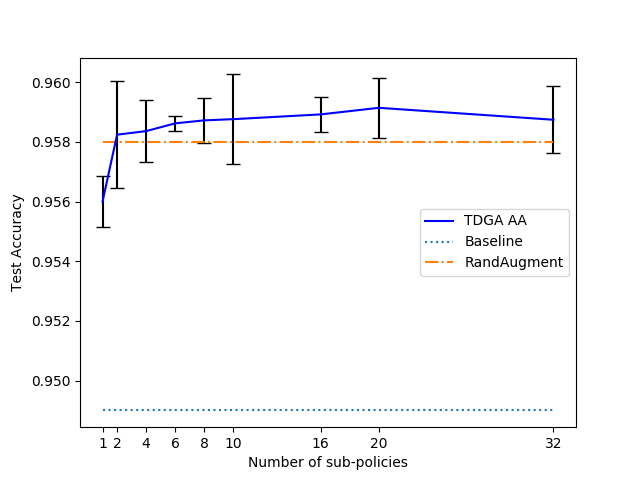
\includegraphics[width=0.7\columnwidth]{figure/exp_change_B.png}
      \caption{最終個体数の変化による識別率の変化}
      \label{fig:change_B}
    \end{center}
  \end{figure}

  \section{エントロピーと最終拡張の選択個数の確認}
  追加資料に記載した最終世代のエントロピーと拡張の選択数の図を更新した.図 \ref{fig:num_operations_t002} に結果を示す.

  \begin{figure}[t]
    \centering
    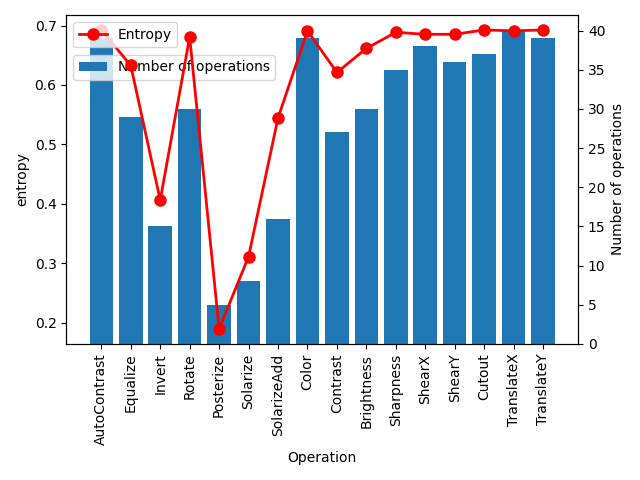
\includegraphics[width=0.8\columnwidth]{figure/num_operations_t002.png}
    \caption{The number of operations in five trials and their entropy values ($T$=0.02).}
    \label{fig:num_operations_t002}
  \end{figure}

  \section{現在できていること}
  \begin{itemize}{
    \item{CIFAR-10 の温度変化,強度変化,個体数変化の結果更新}
    \item{最終世代のエントロピーと得られた拡張の個数の結果更新}
	}\end{itemize}

  \section{できていないこと}
  \begin{itemize}{
    \item{WRN28-10, SVHN に対する精度確認}
    \item{漫画データセットへの適用実験}
    \item{各操作の影響を調べる}
	}\end{itemize}

	% 参考文献リスト
	% \bibliographystyle{unsrt}
	% \bibliography{2020_09_25}
\end{document}
